\chapter{Ewaluacja i rezultaty}
\label{cha:ewaluacjaIRezultaty}
Poniższy rozdział zawiera opis testów przeprowadzonych w celu walidacji działania algorytmu animacji awatara. Przedstawiono w nim również otrzymane rezultaty i wnioski płynące z przeprowadzonych ankiet.

\section{Sposób testowania}
\begin{figure}[h]
	\centering
	\begin{subfigure}{0.35\textwidth}
		\centering
		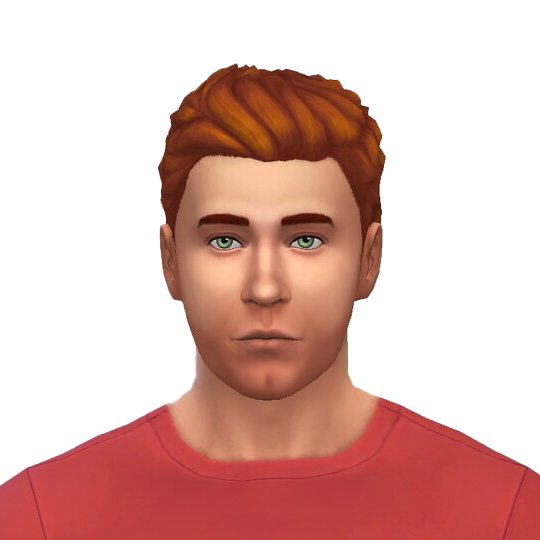
\includegraphics[height=5.5cm]{zdjęcia/1.png}
		\subcaption{\label{avatar_1}}
	\end{subfigure}
	\begin{subfigure}{0.35\textwidth}
		\centering
		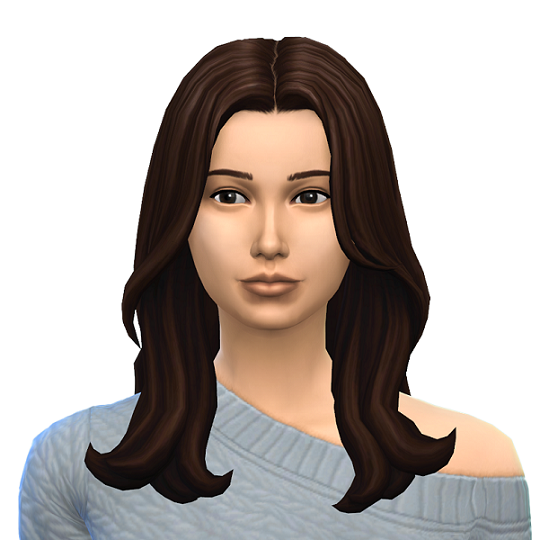
\includegraphics[height=5.5cm]{zdjęcia/2.png}
		\subcaption{\label{avatar_2}}
	\end{subfigure}
	\begin{subfigure}{0.35\textwidth}
		\centering
		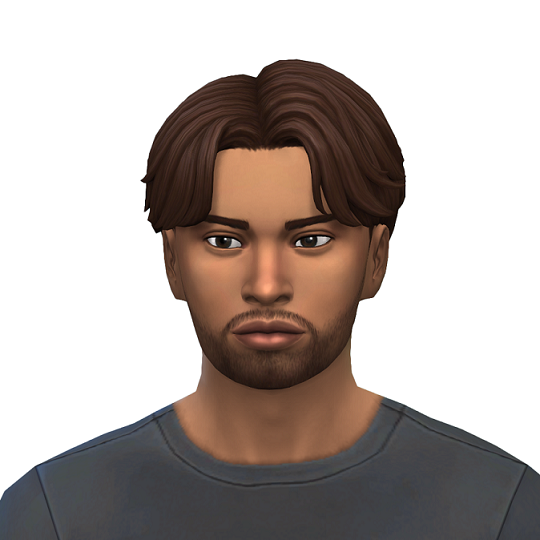
\includegraphics[height=5.5cm]{zdjęcia/3.png}
		\subcaption{\label{avatar_3}}
	\end{subfigure}
	\begin{subfigure}{0.35\textwidth}
		\centering
		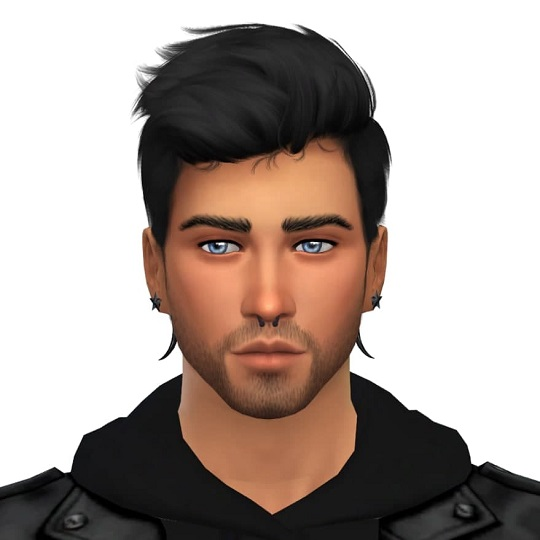
\includegraphics[height=5.5cm]{zdjęcia/4.png}
		\subcaption{\label{avatar_4}}
	\end{subfigure}
	
	\caption{\label{fig:avatars}Awatary użyte do walidacji działania algorytmu}
\end{figure}


\begin{table}
\centering
\begin{tabular}{|c|l|c|c|c|c|c|} 
\hline
\multirow{2}{*}{\textbf{awatar}} & \multicolumn{1}{c|}{\multirow{2}{*}{\textbf{emocja}}} & \multicolumn{5}{c|}{\textbf{ocena}}                                                                                                   \\ 
\cline{3-7}
                                 & \multicolumn{1}{c|}{}                                 & \textbf{1} & \textbf{2} & \textbf{3}                       & \textbf{4}                         & \textbf{5}                          \\ 
\hhline{|=======|}
\multirow{4}{*}{pierwszy}        & szczęście                                             & ~ 0\%~~    & ~ 9\%~~    & ~ 0\%~                           & \textcolor[rgb]{0,0.588,0}{~ 45\%} & \textcolor[rgb]{0,0.588,0}{~ 45\%}  \\ 
\cline{2-7}
                                 & smutek                                                & 0\%        & 0\%        & 0\%                              & \textcolor[rgb]{0,0.588,0}{64\%}   & 36\%                                \\ 
\cline{2-7}
                                 & zaskoczenie/strach                                    & 0\%        & 0\%        & 18\%                             & \textcolor[rgb]{0,0.588,0}{45\%}   & 36\%                                \\ 
\cline{2-7}
                                 & gniew/obrzydzenie                                     & 0\%        & 9\%        & 18\%                             & \textcolor[rgb]{0,0.588,0}{36\%}   & \textcolor[rgb]{0,0.588,0}{36\%}    \\ 
\hhline{|=======|}
\multirow{4}{*}{drugi}           & szczęście                                             & 0\%        & 9\%        & 9\%                              & \textcolor[rgb]{0,0.588,0}{45\%}   & 36\%                                \\ 
\cline{2-7}
                                 & smutek                                                & 0\%        & 27\%       & 9\%                              & \textcolor[rgb]{0,0.588,0}{45\%}   & 18\%                                \\ 
\cline{2-7}
                                 & zaskoczenie/strach                                    & 9\%        & 0\%        & 27\%                             & \textcolor[rgb]{0,0.588,0}{55\%}   & 9\%                                 \\ 
\cline{2-7}
                                 & gniew/obrzydzenie                                     & 9\%        & 18\%       & \textcolor[rgb]{0,0.588,0}{45\%} & 27\%                               & 0\%                                 \\ 
\hhline{|=======|}
\multirow{4}{*}{trzeci}          & szczęście                                             & 0\%        & 0\%        & 9\%                              & \textcolor[rgb]{0,0.588,0}{45\%}   & \textcolor[rgb]{0,0.588,0}{45\%}    \\ 
\cline{2-7}
                                 & smutek                                                & 0\%        & 0\%        & 27\%                             & \textcolor[rgb]{0,0.588,0}{55\%}   & 18\%                                \\ 
\cline{2-7}
                                 & zaskoczenie/strach                                    & 0\%        & 9\%        & 18\%                             & \textcolor[rgb]{0,0.588,0}{36\%}   & \textcolor[rgb]{0,0.588,0}{36\%}    \\ 
\cline{2-7}
                                 & gniew/obrzydzenie                                     & 0\%        & 18\%       & 18\%                             & \textcolor[rgb]{0,0.588,0}{36\%}   & 27\%                                \\ 
\hhline{|=======|}
\multirow{4}{*}{czwarty}         & szczęście                                             & 0\%        & 0\%        & 0\%                              & 18\%                               & \textcolor[rgb]{0,0.588,0}{82\%}    \\ 
\cline{2-7}
                                 & smutek                                                & 0\%        & 9\%        & 0\%                              & \textcolor[rgb]{0,0.588,0}{55\%}   & 36\%                                \\ 
\cline{2-7}
                                 & zaskoczenie/strach                                    & 0\%        & 9\%        & 9\%                              & \textcolor[rgb]{0,0.588,0}{55\%}   & 27\%                                \\ 
\cline{2-7}
                                 & gniew/obrzydzenie                                     & 0\%        & 9\%        & 9\%                              & \textcolor[rgb]{0,0.588,0}{64\%}   & 18\%                                \\
\hline
\end{tabular}
\end{table}



\section{Walidacja działania aplikacji}
% No to tutaj może dla jakichś 15 osób czy coś, poprosić o testowanie i np. osobno te ze zdjęciami a osobno real-time
% szczęście,
% smutek,
% strach/zaskoczenie,
% gniew/obrzydzenie
% No i ocenić to może w skali, czy rezultaty są wystarczające
\section{Ocena osiągniętych efektów}

\begin{figure}[h]
	\centering
	\begin{subfigure}{0.35\textwidth}
		\centering
		
\includegraphics[height=4.5cm]{zdjęcia/av-3_anger_2.png}
		\subcaption{\label{av-3_anger_2}}
	\end{subfigure}
	\begin{subfigure}{0.35\textwidth}
		\centering
		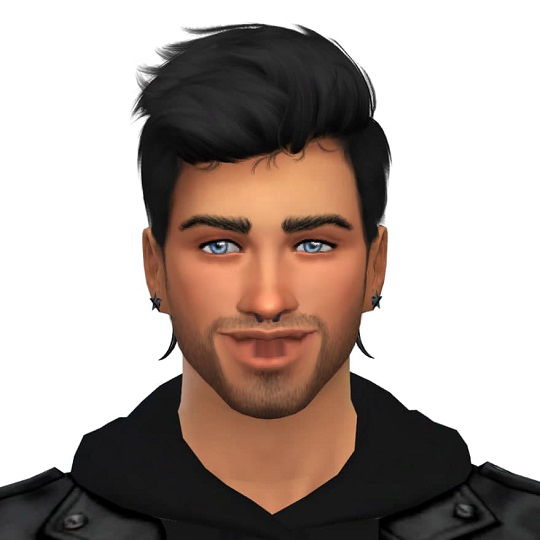
\includegraphics[height=4.5cm]{zdjęcia/av-4_happiness_2.png}
		\subcaption{\label{av-4_happiness_2}}
	\end{subfigure}
	
	\caption{\label{fig:best_results}Najtrafniej odgadnięte odwzorowania}
\end{figure}


\begin{table}
\centering
\begin{tabular}{|c|c|c|c|c|} 
\hline
                                                               & \multicolumn{4}{c|}{awatar}                                                                                                                                                                \\ 
\hline
emocja                                                         & pierwszy                                   & ~ drugi~~                                 & ~ trzeci~~                                          & czwarty                                     \\ 
\hline
szczęście                                                      & ~ 74\%~~                                   & 70\%                                      & 85\%                                                & \textcolor[rgb]{0,0.502,0}{\textbf{100\%}}  \\ 
\hline
smutek                                                         & 78\%                                       & \textcolor[rgb]{0,0.502,0}{\textbf{93\%}} & 85\%                                                & 85\%                                        \\ 
\hline
zaskoczenie/strach                                             & \textcolor[rgb]{0,0.502,0}{\textbf{93\% }} & 74\%                                      & 63\%                                                & 63\%                                        \\ 
\hline
gniew/obrzydzenie                                              & 78\%                                       & 41\%                                      & \textcolor[rgb]{0,0.502,0}{\textbf{96\%}}           & 67\%                                        \\ 
\hline
\bottomrule
\begin{tabular}[c]{@{}c@{}}sumaryczna\\poprawność\end{tabular} & 81\%                                       & {\cellcolor{red}}\textcolor{white}{69\%}  & {\cellcolor[rgb]{0,0.502,0}}\textcolor{white}{82\%} & 79\%                                        \\
\hline
\end{tabular}
\end{table}
% Noo i tutaj sprawdzić np czy działa dla tego szalonego modelu, jeśli tak to sprawdzić jak tam efekty działania aplikacji dla obydwu, można np zestawić z dwóch modeli i kazać ocenić ludziom. Plus jakaś tabelka przedstawiająca porównanie czasu przetwarzania dla kilkunastu obrazów.

% No i we wnioskach to na pewno:
% 1. Jak te modele wypadają na swoim tle, tzn który lepszy i poprzeć wynikami z ankiety
% 2. Przedstawić ocenę aplikacji tej strony real time vs tej z obrazami dwoma
% 3. No i pewnie we wnioskach ze gorzej ta real time dziala, no i ze pewnie trzeba dopracowac i ze tez ma wplyw na to oswietlenie, jakies ustawianie zle twarzy bla bla
